%======================================================================
\subsection{BW-SIM-01 --- Built, 27--30 Oct: static stress end to end, bands and stress measure, LaTeX report}\label{sec:sim01-built}
%======================================================================

Static stress now runs through the whole Simulation workspace. The work is in five commits plus the materials
library: \code{08274d9e} (the headless core, the benchmark, CalculiX in Keystone) and \code{1729f31c} (the
packaging check) on 27 Oct; \code{9750319a} (the workspace GUI and two C++ fixes), \code{ce174d24} (your 30 Oct
answers S1--S4) and \code{e018a43a} (Tectonic in the environment and the bundle) on 30 Oct. The \emph{materials}
agent's \code{9ea0d2ab} added the Keystone material library. The code is in \file{src/Mod/BruceWorx/bruceworx\_sim.py},
which is headless (FreeCADCmd runs it), and \file{bruceworx\_sim\_gui.py} (commands and panels). The questions
S1--S5 of \S\ref{sec:sim01-plan} were built as you answered them: the Keystone library first, bands you can
configure, a stress measure chosen per study, a LaTeX report compiled by a bundled Tectonic, and \code{ccx}
bundled.

\begin{figure}[!htbp]
\centering
\begin{minipage}[b]{0.62\linewidth}\centering
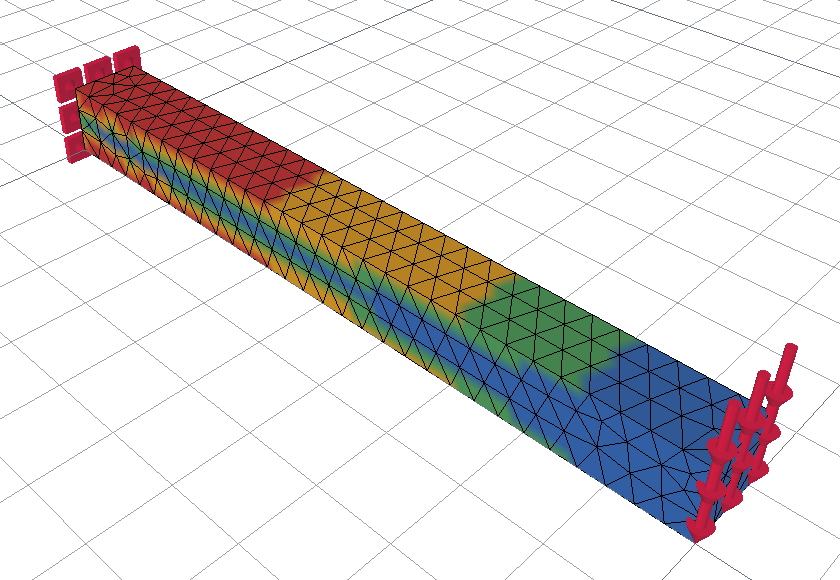
\includegraphics[width=\linewidth]{fig/sim01_safety.png}
\end{minipage}\hfill
\begin{minipage}[b]{0.34\linewidth}\centering
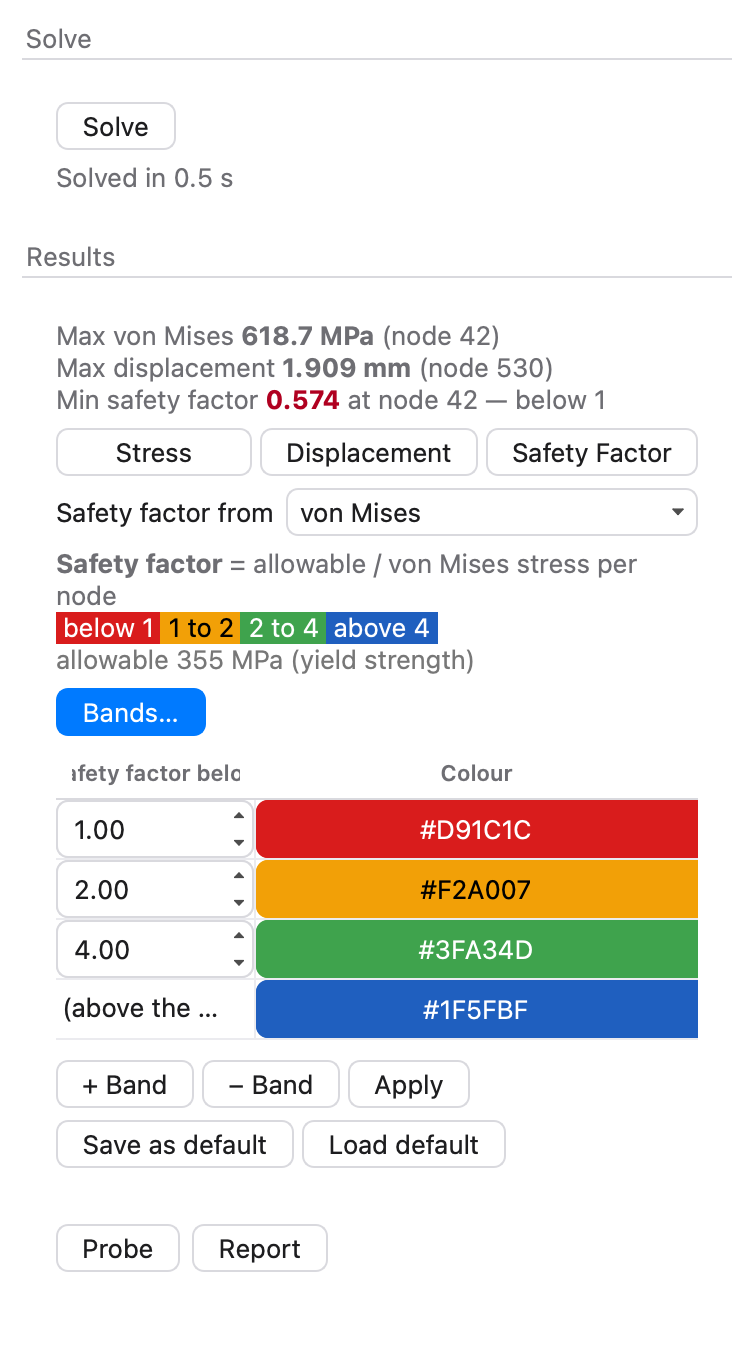
\includegraphics[width=\linewidth]{fig/sim01_panel.png}
\end{minipage}
\caption{Left: the cantilever benchmark (steel, $100\times10\times10$\,mm, 1000\,N at the tip) coloured by
safety factor in four bands set in the study: below 1 red, 1--2 amber, 2--4 green, above 4 blue. Red runs along
the top and bottom fibres near the fixed end, where the bending stress is highest; the neutral axis along the side and the free end stay blue. Right:
the study panel's Solve and Results boxes with the stress measure, the legend and the open band editor. Both
are off-screen renders of the real objects.}
\label{fig:sim01-built}
\end{figure}

\paragraph{What you can do now.}
\begin{itemize}[nosep]
  \item \textbf{New Study} (Simulation $\cdot$ Study, Ctrl+2 for the workspace). Pick the study type: Static stress,
        with Modal, Buckling, Thermal and Thermal stress listed and greyed out as \emph{planned}. Pick the model:
        the selection, the active Body or Part, or every visible solid. The material is prefilled from the part's
        own material. The card list starts with the \textbf{Keystone} library (28 cards, each with a yield
        strength), then the vault's cards, then FreeCAD's own (``FreeCAD (FEM)''), then the rest. A card with
        no yield strength uses its ultimate strength, with a note. A Keystone card marked brittle (acrylic,
        CFRP, G10) gets a hint that the maximum principal measure suits it. Also set the \textbf{stress measure}
        and the mesh: $h=\text{diag}/30$, Moderate, Tet10. \emph{Create study} makes the analysis, the static
        CalculiX solver, the material and the Netgen mesh object, then opens the study panel.
  \item \textbf{The study panel} (Study, or any of Mesh, Pre-check, Solve). The \emph{+ Fixed / Force /
        Pressure / Displacement} buttons open the stock FEM panels and return to this panel when they close.
        A double-click on a load or constraint edits it. \emph{Pre-check} lists what a solve still needs:
        material, supports (with a test for rigid-body motion), loads, empty references, zero loads and
        \code{ccx}. \emph{Mesh} and \emph{Refine} (element size $\times0.7$) show the node and element counts.
        \emph{Solve} meshes if needed and runs \code{ccx} in a separate process, so the window stays usable;
        it then reads the results and computes the safety factor. The results summary gives the maximum von
        Mises stress, the maximum displacement and the minimum SF, each with its node.
  \item \textbf{Fields.} \emph{Stress} and \emph{Displacement} (with exaggerated displacement) colour the result
        mesh from blue to red. \emph{Safety Factor} draws the study's bands, with the legend in the panel.
  \item \textbf{Bands} (S2). The panel's \emph{Bands\dots} button, or \emph{SF Bands} in the ribbon, opens the
        editor: one row per band (its upper safety factor and its colour). \emph{+ Band} and \emph{-- Band} add
        or remove a band, so there can be any number. \emph{Apply} sets the bands on the study (properties
        \code{SFThresholds} and \code{SFColors}); the mesh and the legend follow at once. \emph{Save as default}
        writes them to the preference \code{Mod/BruceWorx/Sim} (\code{SFThresholds} \code{"1;2"},
        \code{SFColors} \code{"\#D91C1C;\#F2A007;\#3FA34D"}), and new studies start from it. Thresholds that
        do not rise from band to band are refused, and the panel says why.
  \item \textbf{Stress measure} (S3). The study's \code{StressMeasure} is \emph{von Mises} (the default, also
        a preference), \emph{Maximum principal (Rankine)}, $\sigma_{eq}=\max(|\sigma_1|,|\sigma_3|)$, or
        \emph{Tresca}, $\sigma_{eq}=\sigma_1-\sigma_3$. When you change it in the panel, the safety factor is
        recomputed from the principal stresses already stored on the result, with no new solve. The result
        records the measure it used (\code{StressMeasure}, \code{MaxEquivalentStress}), and the legend and the
        report name it.
  \item \textbf{Probe.} Click a point on the result mesh. The panel shows the nearest node's von Mises stress,
        displacement and safety factor.
  \item \textbf{Report} (S4), written when you ask for it. It writes
        \file{<document>\_<study>\_report/report.tex} with three off-screen renders (\file{fig\_stress},
        \file{fig\_displacement}, \file{fig\_safety}) beside the document. For a vault file that is the vault
        item's working folder. It then compiles \file{<document>\_<study>\_report.pdf} next to the folder, in
        the background, and the panel shows a link when the PDF is done. The report covers: the study, the
        material with the allowable stress and its basis (with a note when it comes from the ultimate
        strength), the mesh, supports, loads, results, the measure and its formula, the band table with node
        counts, the figures, the pre-check, and a line saying the SIM-04 convergence study was not run.
        Without a LaTeX compiler, the \file{.tex} folder stays and the panel says so.
\end{itemize}

\paragraph{The cantilever benchmark} (\eref{SIM-05}'s first case, in \file{TestBruceWorxSimCore}). Steel with
$E=210$\,GPa, $\nu=0.3$ and $\sigma_y=355$\,MPa; the beam is $100\times10\times10$\,mm, fixed at one end, with
$P=1000$\,N at the free end. The default mesh has 2955 nodes and 1581 Tet10 elements at $h=3.37$\,mm.
\begin{center}
\small
\begin{tabular}{@{}lll@{}}
\toprule
Quantity & FE & Theory, note\\
\midrule
Tip deflection & 1.9087\,mm & $PL^3/3EI=1.9048$\,mm (0.21\,\%)\\
Max von Mises & 618.7\,MPa & $Mc/I=600$\,MPa (3.1\,\%, root corners)\\
Max Tresca $\sigma_1-\sigma_3$ & 631.4\,MPa & \\
Max $\max(|\sigma_1|,|\sigma_3|)$ & 815.8\,MPa & at the fixed corners\\
\midrule
Min SF: von Mises, Tresca, Rankine & 0.574, 0.562, 0.435 & $355/\sigma_{eq,\max}$\\
Nodes per band (edges 1, 2, 4) & 443, 750, 649, 1113 & red, amber, green, blue\\
\bottomrule
\end{tabular}
\end{center}
The beam theory is matched to 0.2\,\% in deflection. The Rankine value is far above the bending stress because
of the boundary condition, not the material. A fully fixed face also stops the face's Poisson contraction, so
the stress state at its corners is triaxial and has a large hydrostatic part: $|\sigma_1|$ grows there while
von Mises, which ignores hydrostatic stress, hardly changes. This is a singularity, so a finer mesh makes it
larger (\eref{SIM-04}). Question~2 below asks how to handle it.

\paragraph{Decided while building.}
\begin{itemize}[nosep]
  \item \textbf{Default bands: 1 and 2} (red, amber, green), as the plan recommended. The five bands of the
        27 Oct build (1, 1.5, 2, 4) are one \emph{+ Band} away. The bands belong to the study, not the result,
        so a new solve keeps them. The colours are stored as \code{\#RRGGBB} strings, which are readable in
        the property editor.
  \item \textbf{Rankine is $\max(|\sigma_1|,|\sigma_3|)$}: compression counts by its magnitude, and the report
        says so. For printed plastics, which are stronger in compression, this errs on the safe side.
        \textbf{Tresca} uses $\sigma_1-\sigma_3$ against the yield strength, which is the same as comparing the
        maximum shear stress with $\sigma_y/2$. A result without principal stresses falls back to von Mises
        and records that it did.
  \item \textbf{Band colours are per node.} The mesh view provider shades smoothly between nodes, so a band
        edge is blurred across one element rather than drawn as a sharp $SF=1$ line. A sharp contour needs the
        VTK pipeline, which still crashes in this build (see the next item), or colouring per element (question
        1). Found while making the figure: \code{NodeColor} only fills \code{NodeColorArray}, and the mesh paints
        it only in the \code{ByNode} colour mode. The safety field now sets that mode, and the stress and
        displacement fields set it back to \code{Overall}.
  \item \textbf{Two C++ fixes} (\code{9750319a}), without which no FEM mesh could be created in the GUI while a
        Python document observer was installed. \code{ViewProviderFemMesh} now sets its appearance after its last
        \code{ADD\_PROPERTY}. \code{DocumentObserverPython::slotChangedObject} skips a view provider that is not
        yet attached to its object. Separately, the FRD import's VTK post pipeline is suppressed while a study
        loads its results: creating a \code{Fem::FemPostPipeline} here crashes in
        \code{SoFCColorGradient::setMarkerLabel}.
  \item \textbf{The report.} The HTML and Qt-printer report was removed rather than kept as a fallback. The
        LaTeX template needs only \code{iftex}, \code{fontspec} (under \code{pdflatex}: \code{inputenc},
        \code{fontenc} and \code{lmodern}), \code{geometry}, \code{graphicx}, \code{booktabs} and \code{xcolor},
        so it compiles under Tectonic (XeTeX), \code{latexmk} and \code{pdflatex}. Compilers are tried in this
        order: the preference \code{TexPath}, Tectonic in \file{Contents/bin}, in the pixi environment, on
        \code{PATH}, then \code{latexmk} and \code{pdflatex} on \code{PATH} or in \file{/Library/TeX/texbin}.
        A report written headless has no renders and says so. Fixed on the way: every number of 100 or more
        printed as ``$>100$'' (the safety-factor cap was applied to all values), so $E$ showed as ``$>100$\,MPa''.
  \item \textbf{Tectonic} (\code{e018a43a}) was added to \file{pixi.toml} the way \code{calculix} is. The lock gained
        only the \code{tectonic} package on each platform. \file{make-keystone.sh} copies it into
        \file{Contents/bin}, and \file{keystone\_relocate.py} brings its 12 dylibs (ICU, HarfBuzz, graphite2,
        FreeType, libpng, zlib, iconv, glib, libc++); this was tried on a small test bundle with an empty
        environment. \textbf{Its first run needs the network}: it downloads about 40\,MB of TeX files into
        \file{\textasciitilde/Library/Caches/Tectonic}, which takes about 30\,s. After that it compiles offline
        in a second or two. The cache is not pre-seeded in the bundle (question 3).
  \item \textbf{Brittle cards get a hint, not an automatic switch.} You chose von Mises as the default per study;
        choosing the measure from the material's class is \eref{SIM-03}'s.
  \item \textbf{Room for modal and buckling.} The study's type is the \code{StudyType} property. The type list
        (\code{STUDY\_TYPES}) marks each type as available or planned, and only \code{new\_study}'s solver setup
        and the safety factor assume a static study. A modal or buckling study adds its own solver settings
        (CalculiX \emph{frequency} or \emph{buckle}) and result view on the same panel, mesh, material, report
        and workspace.
\end{itemize}

\paragraph{Tests.} Headless (\file{TestBruceWorxSimCore}, 24). Material cards: Keystone first, every Keystone card
with a yield strength. The allowable stress (yield, then UTS, then none). The study's defaults: measure, bands,
a refused unknown measure. The pre-check. Tet10 meshing and refining. The LaTeX report of an unsolved study,
compiled with Tectonic to a PDF beside the given folder. TeX escaping. Principal stresses of three tensors. One
test per measure on a result built by hand, with 200\,MPa yield: pure shear $\tau=50$ gives SF $2.31/2.0/4.0$
(von Mises/Tresca/Rankine); uniaxial 100 gives 2.0 under all three; $(100,0,-50)$ gives $1.51/1.33/2.0$.
Band validation, band indices, labels and counts. The bands preference: saved, read back, and the built-in
default when the preference is broken. The cantilever above, with all three measures. GUI
(\file{TestBruceWorxSimulation}, 6, under \file{run\_gui\_tests.py}): the commands; New Study (planned types
disabled, the library headings with Keystone first, the measure, \emph{Create}); the part's material
prefilled; the pre-check refusing a study without a load; the solve, the band colours on the mesh, the switch
to Tresca, the band editor (add, colour, apply, refuse, remove, save as default), the probe, and the report
with three figures compiled to a PDF; the five Results commands in the ribbon. \file{TestBruceWorxWorkspaces}
(25), the connection lint in \file{TestBruceWorx} and \file{TestBruceWorxMaterials} (8) also pass.

\paragraph{Open questions for you.}
\begin{enumerate}[nosep]
  \item \textbf{Sharp band edges.} The safety-factor bands blur across one element because the mesh shades
        smoothly between nodes. Colour each element by its lowest node SF instead, for crisp but slightly
        blocky bands, or keep the smooth version?
  \item \textbf{Constraint singularities.} A fully fixed face produces a stress peak at its corners. This peak
        sets the minimum SF under Rankine (0.435 against 0.574 for von Mises on the benchmark) and grows as the
        mesh is refined. Report it as it is, mark nodes on fixed faces as ``at a support'' in the summary and
        the report, or leave them out of the minimum (Fusion has an option for this)?
  \item \textbf{Tectonic offline.} Pre-seed its cache: about 40\,MB in \file{Contents/Resources}, copied to
        \file{\textasciitilde/Library/Caches/Tectonic} on first use, so the first report also works without a
        network. Or keep the one-time download?
  \item \textbf{The report in the vault.} The PDF sits beside a vault file in the item's working folder. Should
        it also be checked in as an attachment of the item, so a release package (\eref{PDM-05}) carries it
        automatically?
  \item \textbf{A preferences page.} The default bands and the measure are set from the study panel (\emph{Save as
        default}) and stored in \code{Mod/BruceWorx/Sim}. Add a Simulation page to Preferences for them, the
        compiler path and the mesh divisor?
\end{enumerate}
